\documentclass[twocolumn]{article}
\usepackage[utf8]{inputenc}
\usepackage{graphicx}
\usepackage{gensymb}
\usepackage[]{booktabs}

\title{Braess's Paradox}
\author{Nick Benitez}

\date{\today}

\begin{document}
\begin{titlepage}
	\maketitle
	\tableofcontents
\end{titlepage}

\begin{abstract}
Braess's Paradox, first described by Dietrich Braess in 1968, is a counterintuitive phenomenon in network theory where adding extra capacity to a system can paradoxically reduce overall performance. This occurs when self-interested agents optimize their own paths, leading to a suboptimal Nash Equilibrium compared to the social optimum. While the paradox is commonly illustrated through traffic networks, this paper explores it mechanically using a spring-based countersnapping mechanism, drawing analogies to Hooke's Law and extending the concept to fields such as fluid dynamics, electron movement, and electrical circuits.

The study details the design, 3D printing, and assembly of a prototype using Thermoplastic Polyurethane (TPU) and Polylactic Pcid (PLA), based on Paul Ducarme's open-source model. Experimental procedures involve measuring spring constants and testing the mechanism under incremental loads to observe the transition from series to parallel configurations. Results demonstrate the snap-through behavior, though material limitations prevent perfect alignment with theoretical predictions. Data analysis reveals a force threshold for configuration change, validating the paradox's principles despite deviations due to fabrication constraints. Future work suggests exploring analogous behaviors in electrical circuits and capacitive networks.
\end{abstract}


\section{Introduction}
Braess's Paradox, first proposed by economist Arthur Pigou and later named mathematician Dietrich Braess in 1968, describes a counterintuitive phenomenon in network theory: adding extra capacity to a network has the ability to decrease the overall performance of the system. This occurs when items in the system act "selfishly" to optimize their own utility, leading to a suboptimal \textbf{Nash Equilibrium} \cite{braess}.

\subsection{Mechanically}
While commonly explained through traffic \cite{pas1997braess}, I find it easier to explain the system of springs and strings.

Consider a weight supported by two identical springs, each with a spring stiffness ($K_1$,$K_2$)and two long pieces of string ($T_1, T_2$). Initially, the springs are connected in a configuration where they are under high tension. Consider the Hooke's law equations 1 and 2 \cite{hooke1678spring}:
\begin{equation}
	K_1+K_2=K_{parallel} 
\end{equation}
\begin{equation}
	\frac{1}{K_1}+\frac{1}{K_2}=\frac{1}{K_{{series}}}
\end{equation}

If a new, short connecting string is added between the springs, one might assume it provides more support. However, it can cause the weight to hang lower as the system transferred from in series to in parallel. Conversely, cutting a connecting string can cause the weight to rise, as the load redistribution forces the springs into a parallel configuration \cite{penchina2003braess}. 

\subsection{The Mathematical Framework}
The paradox is defined by the gap between the {Social Optimum} (the configuration that minimizes total system cost) and the {Nash Equilibrium} (where no individual can improve their position by changing strategy alone).

In a network with total flow $R$, if $c_e(f_e)$ is the cost function of an edge $e$ with flow $f_e$, the Nash Equilibrium occurs when all used paths $P$ have an equal and minimal cost:
\begin{equation}
\sum_{e \in P} c_e(f_e) = L
\end{equation}
The {Price of Anarchy} (PoA) quantifies this inefficiency:
When Braess's Paradox occurs, adding an edge increases the cost of the Nash Equilibrium while the Social Optimum remains the same or decreases.

\begin{equation}
	PoA = \frac{\textbf{Cost of Nash Equilibrium}}{\textbf{Cost of Social Optimum}}
\end{equation}

\section{My process}

The creator of the mechanism, Paul Ducarme, mentions on his project website that the initial model was cast with silicone in a printed mold. I chose to print the models directly as that allows time in my independant study to have quick prototypes so it doesn't require reprinting and waiting for silicone to cure.

My final countersnapping structure had been printed out of thermoplastic polyurethane (TPU). With more experimental time, flexible resin would have much higher quality and repeatable print though I've had minor success out of it as I've found it to be "spongey" in elasticity rather than "snappy". Perhaps mixing the material with a stiffer resin would make it better for this application.

\subsection{Printing}

I started out by skimming the supplimentary information paper and downloading the countersnapping files from the project website \cite{ducarme_projects_countersnapping_structure}. Inside the .zip file contains 3 folders: Connectors, Molds, and Parts. For my build I only used models from the Connectors and Parts directories. From the project site, Ducarme directed to create the parts listed:
\begin{itemize}
	\item[] {2 stiffening blocks}
	\item[] {1 non-monotonic block}
	\item[] {2 softening blocks}
	\item[] {2 outer connectors}
	\item[] {2 inner connectors }
\end{itemize}
I took files and imported the models in my GCode slicer of  choice: the open source edition of Ultimaker Cura.

\begin{figure}
	\centering
	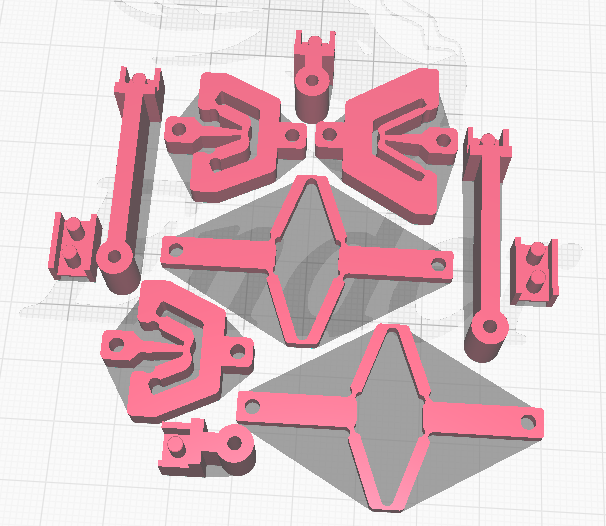
\includegraphics[width=0.5\linewidth]{557117BB-BA0D-4337-9833-3D22AEFEB5C3.png}
	\caption{Lineup of all needed files in a 3d printing slicer software.}
	
	\label{fig:slicer}
\end{figure}

An important note is that it's ideal to print all parts flat as seen in Figure \ref{fig:slicer}. This prevents the layer lines creating weaker links in the parts. Here are some settings in Cura that I've found to be useful in this build:

\begin{itemize}
	\item[] Layer height: $.16 mm$
	\item[] Bed temp: 70 $\degree C$
	\item[] Hotend Temp: 210 $\degree C$
	\item[] Enable Print Ironing: True
	\item[] Fan Speed: $50\%$
\end{itemize}

\subsection{Assembly}

\begin{figure}
	\centering
	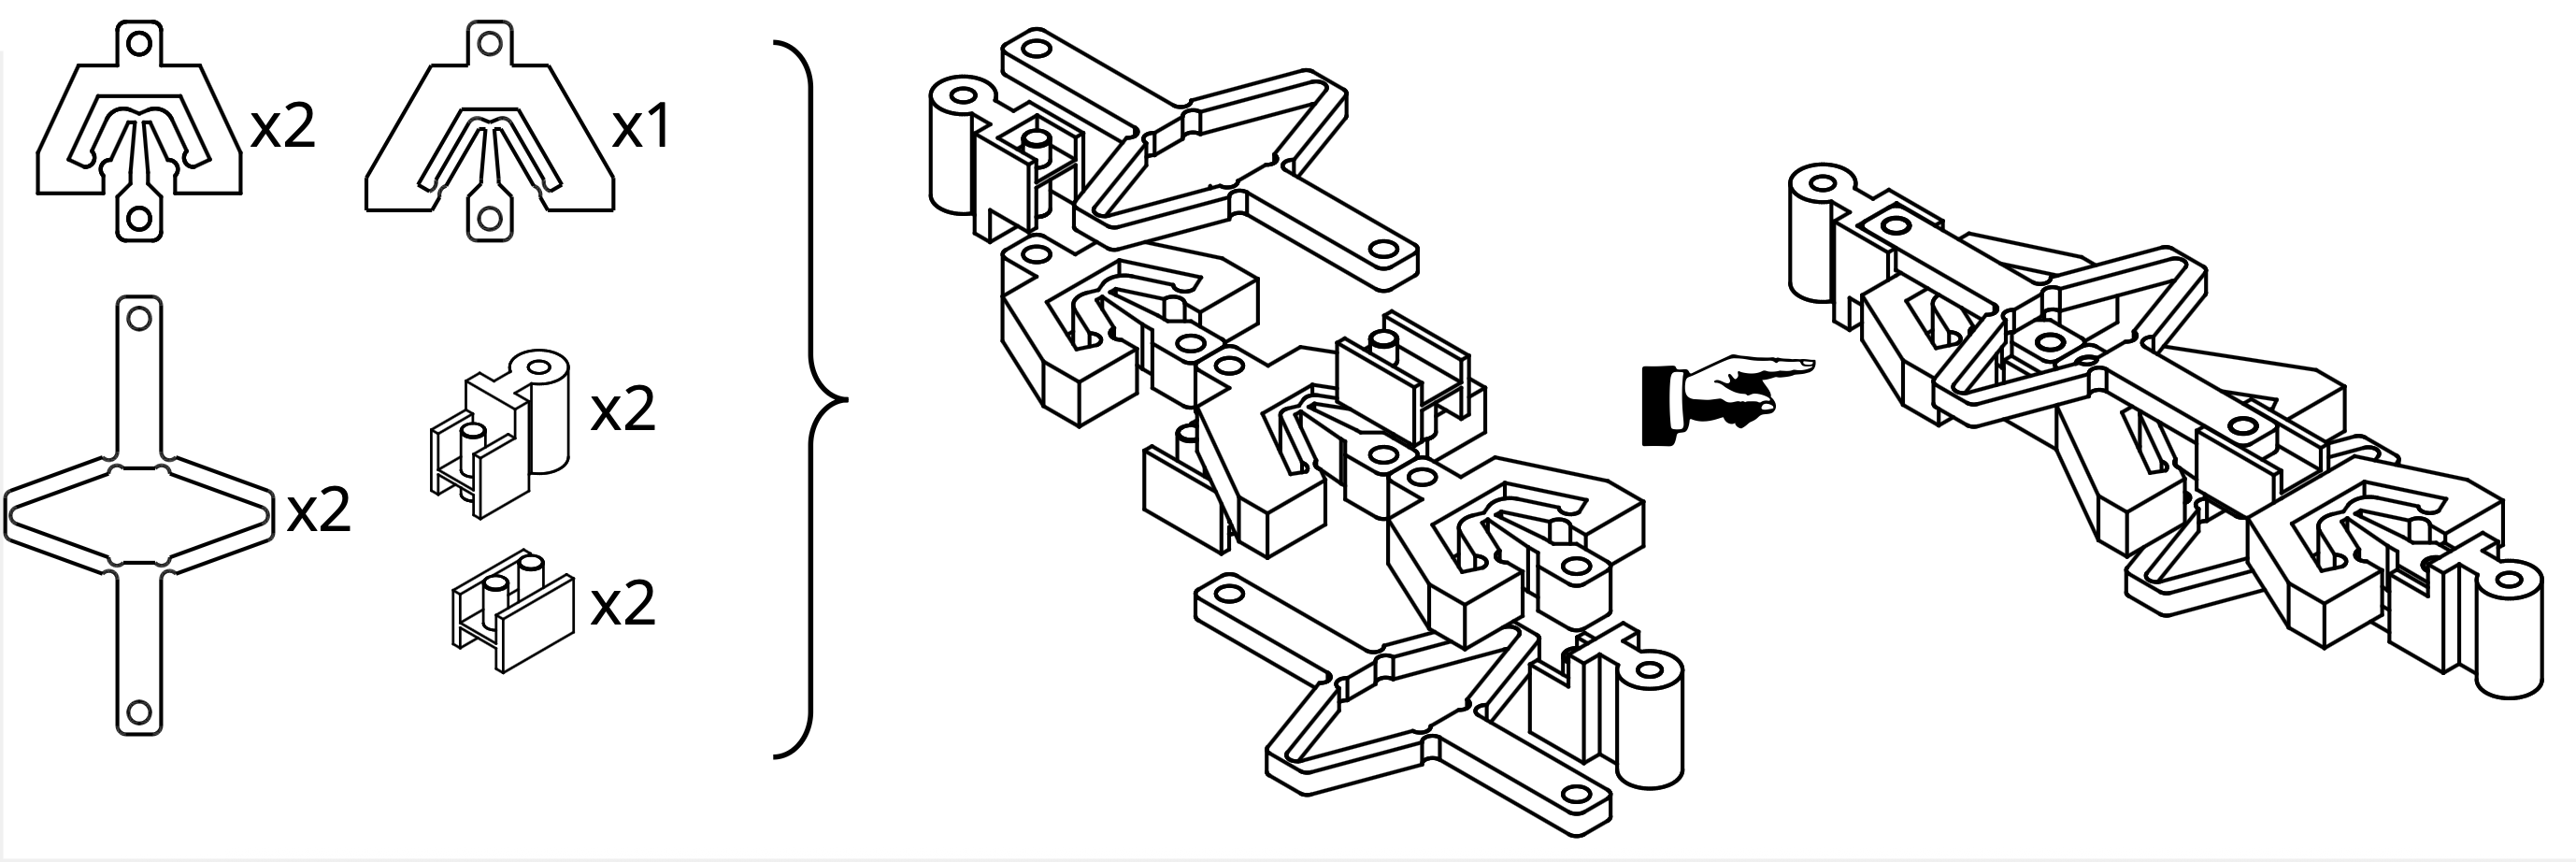
\includegraphics[width=1\linewidth]{howto}
	\caption{A diagram demonstration on the orientations and positions of each piece of the assembly. \cite{ducarme_projects_countersnapping_structure}}
	\label{fig:diagram}
\end{figure}

I assembled the required flexible spring parts in reference to Figure \ref{fig:diagram} out of TPU, and the links out of PLA for stiffness. The full assembly is shown in Figure \ref{fig:device}.

\begin{figure}
	\centering
	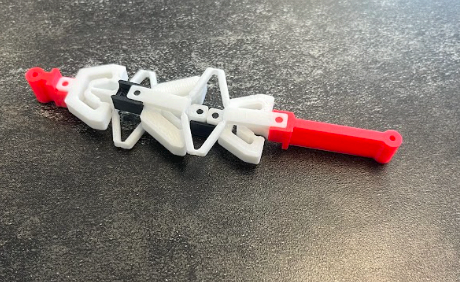
\includegraphics[width=.9\linewidth]{device}
	\caption{The device consisting of 4 springs and one switch made of white TPU and linkages as standard PLA plastic.}
	\label{fig:device}
\end{figure}

\subsection{Problems encountered}
 I had a problem at first printing the linkages in flexible TPU but that resulted in problematic unneeded flexibility so I ended up printing the links in standard Creality PLA. Even then I found them to be quite fragile and brittle, as their size compromises the structure of the layer lines. The links work fine but replacing parts often requires the links to reprinted so I made 20 extra.
 
 To build a proper model it would be better to make it out of silicone like the original. No other material found that can be 3d printed beats the near perfect elasticity of silicone and TPU only made a model that can only sort of show the paradox. Basically, TPU wont have the countersnapping result desired. 

\section{Testing Hooke's law edition of Braess' paradox}

This mechanism consists of 3 different types of springs: Stiff, Soft, and Snapping. To measure the k values of each spring, I took paperclips to the end loops of each part and clamped them in a hobbiest vice over open air letting the spring dangle and measured the distance of the spring loops at rest with a plastic bag hanging as a basket for inserting quarters as weights. In this experiment the mass of a single quarter is $5.67 grams$, and the force applied in a downward direction for each quarter in a basket is $55.62$ Millinewtons of force. So for every \$0.25 it is equal to $55.62$ mN. Table \ref{tab:spring_data} provided has the average distances for each spring applied with a dollar (222.48 mN).

\begin{table}[h]
	\centering
	\caption{Spring Characteristics Under Applied Force}
	\label{tab:spring_data}
	\begin{tabular}{lccc}
		\toprule
		Spring & Rest (mm) & Distance (mm)  & $k\frac{N}{m}$ \\
		\midrule
		Stiff & 19.4 & 19.9 & 111.24 \\
		Soft & 46.2 & 53.9 & 1713.096 \\
		Snap & 17.5 & 18.2 & 155.736 \\
		\bottomrule
	\end{tabular}
\end{table}

Measured; the 2 outer weak springs have a Hooke's constant ($k$) of $28.89 \frac{ N}{m}$ and the inner strong springs have a $k= 444.96 \frac{ N}{m}$. The middle snapping structure is a spring of $k= 317.83 \frac{ N}{m}$.

\subsection{Theoretically}
This mechanism would be represented by 5 springs. In the unsnapped position, the active springs would be the 2 stiff and lone snapping springs in order such that they are in series, visualized in the diagram. 

\begin{center}
	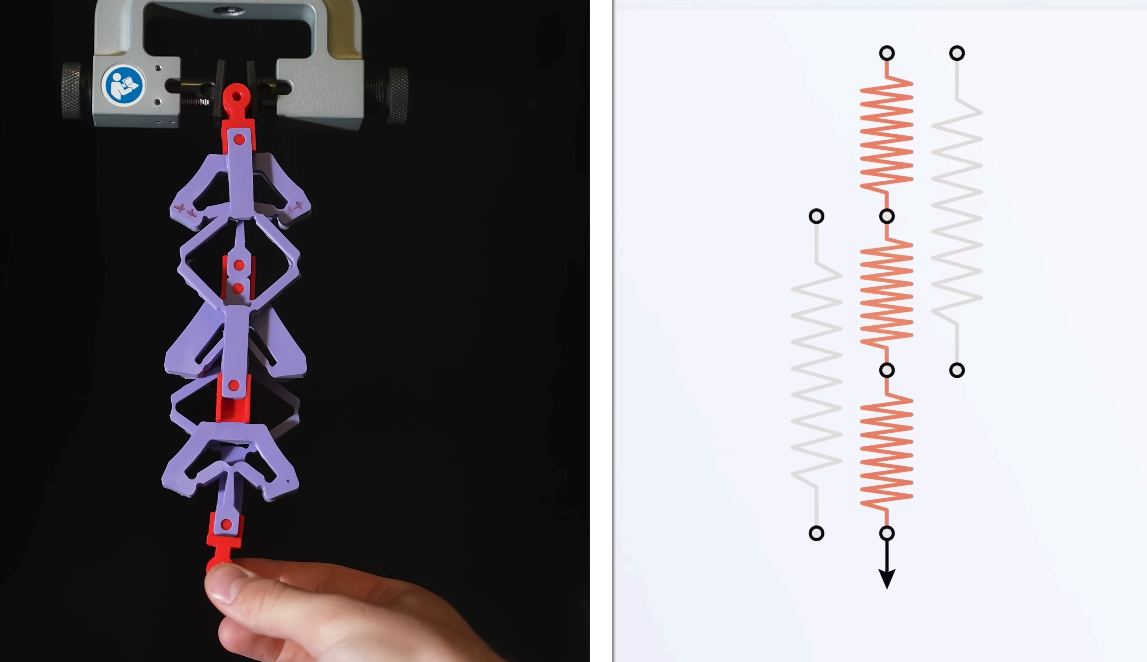
\includegraphics[width=0.4\textwidth]{Screenshot_20260420_134704}
\end{center}

When stretched, the middle link "snapps" out to expose a different organization to the mechanism at rest. This action swaps the springs from in series to in parallel, "shrinking" the mechanism when force is applies outward.

\begin{center}
	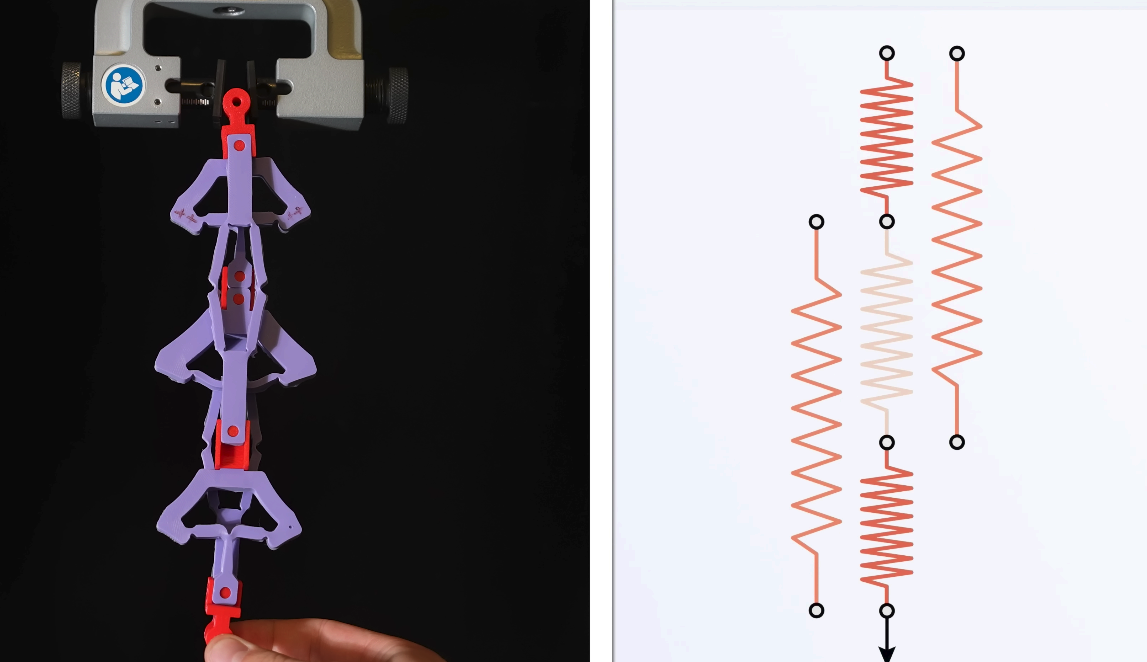
\includegraphics[width=0.4\textwidth]{Screenshot_20260420_134726}
\end{center}

\cite{veritasium_countersnapping_2025}. 

Doing the series vs parallel math of each diagram representing each spring leads to the theretical k values:
$k_{unsnapped}= 130.87 \frac{N}{m}$ snapping to $k_{snapped}=54.25 \frac{N}{m}$.

We can utilize the $k$ constants to calculate the theoretical distance traveled with a certain amount of force applied utilizing Hooke's Law. 

\begin{equation}
	\frac{\textbf{Force Applied}}{k} = \textbf{Distance}
\end{equation}

Implementing the $k$ constants to this equation and graphing them in relation to the force applied will result in 2 linear functions (See Figure \ref{fig:graph}). 

\begin{figure}
	\centering
	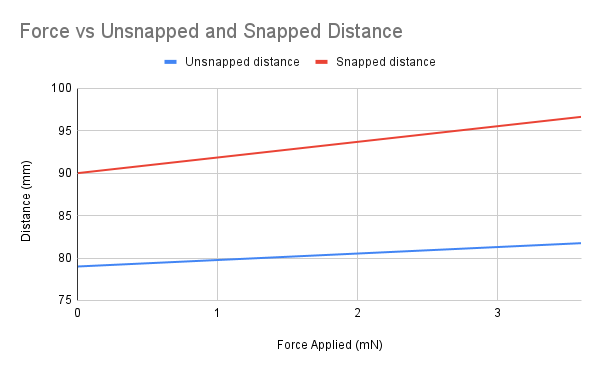
\includegraphics[width=1\linewidth]{Force vs Unsnapped and Snapped Distance}
	\caption{2 linear functions showing the theoretical relation of force applied versus mechanism distance. This shows how the mechanism in the second, "snapped", function will always remain to the left the first, "unsnapped", configuration with the same force applied.}
	\label{fig:graph}
\end{figure}

One would notice later in the paper this graph is innacurate, since the unsnapped distance is always less than the snapped distance, making the mechanism shoot forward when enough force is applied to flip the nonmonotonic part to the second configuration. This is unlike the structure described at the beginning of this section, this is due to several reasons:

\begin{enumerate}
	\item The original mechanism was made out of silicone, and unfortunately I don't have the time to work with that material.
	\item TPU is still too spongey to be utilized well in this application. 
	\item The resting distance of the unsnapped configuration is 79 mm, whereas the rest distance of the latter is 90 mm.
	\item The final prototype could not achieve greater total stiffness in the snapped configuration, which is essential for the countersnapping effect to function as designed.
	
\end{enumerate}

This doesn't mean the total build is a failure, though, as this experiment can still demonstrate when Braess's paradox occures.

\subsection{Experiment Procedures}
For this experiment I have materials and tools in my home lab that I found useful:
\begin{itemize}
	\item[] {a hobby vice clamp,}
	\item[] {paper clips,}
	\item[] {an elevated surface (like a desk),}
	\item[] {small plastic bags,}
	\item[] {an array of coins (or some type of weight),}
	\item[] {a pair of digital calipers,}
	\item[] {and a digital cooking scale.}
\end{itemize}

I begin by installing the vice grip to the end of an elevated surface in my bedroom lab and clamping the top of the mechanism letting the device hang freely.


\begin{figure}
	\centering
	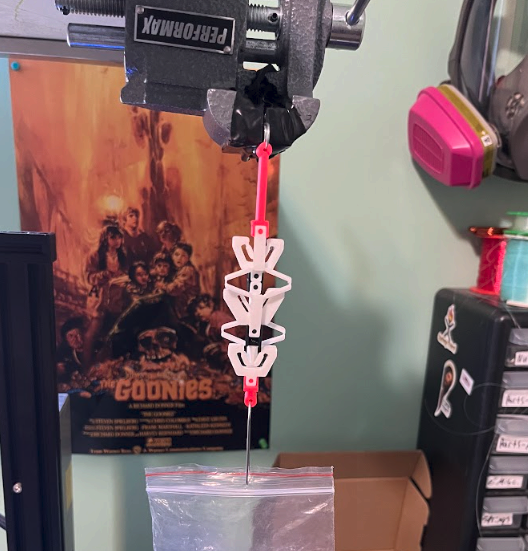
\includegraphics[width=.9\linewidth]{setup}
	\caption{The device hanging from a paperclip clamped by a desk vice, with another paperclip on the other end holding up a plastic bag.}
	\label{fig:setup}
\end{figure}

I poke a paper clip through a plastic bag and thread the paperclip through the lower end of the mechanism, I now have a basket. I measure the device in this setup with the pair of calipers without any extra weight in the bag (See Figure \ref{fig:setup}). This is the rest distance applied in Table \ref{tab:mass_distance}.

I added coins incrementally and measured the mechanism's distance after each addition. The weight values in Table \ref{tab:mass_distance} were calculated using the gravitational acceleration constant of $9.81 \, \frac{{m}}{{s}^2}$ multiplied by the mass in grams. Notably, no significant deformation occurred until the applied weight reached approximately 150 grams.

\begin{table}[h]
	\centering
	\small
	\caption{Mass Applied vs. Experimental Distance}
	\label{tab:mass_distance}
	\begin{tabular}{ccc}
		\toprule
		Mass (g) & Weight (mN) & Distance (mm) \\
		\midrule
		0 & 0 & 79 \\
		34 & 0.33354 & 79 \\
		99 & 0.97119 & 80 \\
		188 & 1.84428 & 81 \\
		275 & 2.69775 & 83 \\
		309 & 3.03129 & 85 \\
		318 & 3.11958 & 96 \\
		322 & 3.15882 & 96 \\
		336 & 3.29616 & 97 \\
		363 & 3.56103 & 97 \\
		\bottomrule
	\end{tabular}
\end{table}

Figure \ref{fig:experiment_graph} displays the experimental data overlaid with the theoretical linear functions. The data initially follows the unsnapped distance trendline closely, then sharply transitions and plateaus at 97 mm, the maximum stretched length of the device. This behavior demonstrates that the mechanism does undergo a configuration change, though not in the ideal manner predicted by theory. The transition occurs at approximately 3.1 mN of applied force, where the mechanism snaps into its second state. A more precisely engineered prototype would better align with theoretical predictions and would illustrate Braess's paradox better.

\begin{figure}
	\centering
	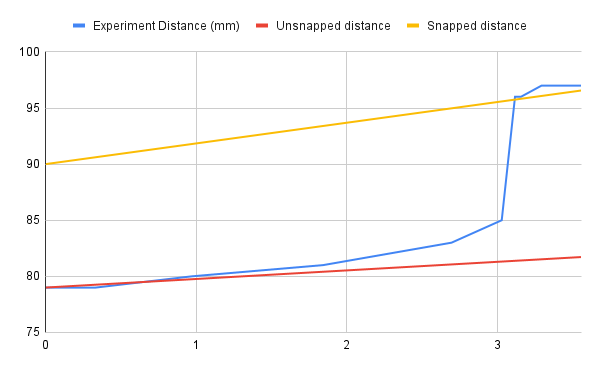
\includegraphics[width=1\linewidth]{Force vs Distance with Linear Function Overlay}
	\caption{Experimental data overlaid with theoretical linear functions representing unsnapped and snapped configurations. The initial trend closely follows the unsnapped distance trendline until the mechanism snaps and follows the other trendline until it plateaus at 97 mm, which represents the maximum stretched length of the device.}
	\label{fig:experiment_graph}
\end{figure}

Braess's paradox occurs when adding a new element (like a road or spring in parallel) to a system actually decreases overall performance. In this case, it would mean that the snapped configuration (with springs in parallel) should theoretically allow less extension under the same force, but the data shows the opposite happening initially.

The parallel configuration should be stiffer because it has a higher k value, but the unsnapped resting distance of 79 mm vs. snapped resting distance of 90 mm means the mechanism actually becomes less stiff. This make it not exactly a good example of Braess's paradox in action, but still has potential for future developement as this would be what I consider, entirely human error.

\section{Conclusion}

This investigation explored the countersnapping mechanism as a mechanical manifestation of Braess's paradox, demonstrating how a system can behave counterintuitively when its configuration changes. The observed mechanism composed of springs in series can transition to a parallel configuration, fundamentally altering its response to applied force. While the prototype did not achieve the idealized behavior predicted by theory due to material limitations and design constraints, it successfully illustrated the snap-through transition and provided empirical evidence of configuration-dependent stiffness.

The experimental data in Table \ref{tab:mass_distance} revealed that the mechanism exhibits a sharp transition at approximately 3.1 mN of applied force, transitioning from the unsnapped to snapped state and plateauing at a maximum extension of 97 mm. This behavior, though not perfectly aligned with theoretical predictions, validates the fundamental principle that mechanical systems can exhibit paradoxical responses when structural constraints change.

\subsection{Future experimentation}
This phenomina is experienced in a wide range of fields such as electron movement, logistics, and fluids to name a few. 

During the research for this study, I found a paper sourcing a circuit \cite{Nagurney2016Braess} that was utilized to measure resistance in a circuit. I created a quick simulation to mimic Nagurney's paper in the software SimulIDE and found similar results to Nagurney's collected data (See Figure \ref{fig:simulation}). 

I would imagine a proper experiment with physical hardware would be insightful in how resistors function fundimentally. Perhaps if resistors could show how electrons flow in this counterintuitive way, maybe it would be similar to transition to experimenting with capacitors, as they also function differently in series vs in parallel. By measuring actual voltage drops and current flow across different circuit topologies, one could directly observe how electrons navigate these counterintuitive pathways, including capacitive systems, which exhibit analogous but distinct series and parallel behavior. Since capacitors combine inversely to resistors capacitance increases in parallel but decreases in series. Exploring whether Braess's paradox manifests in capacitive networks could show whether this phenomenon is universal for networked systems or specific to certain types of elements. 

In conclusion, this work demonstrates that Braess's paradox is not merely a theoretical curiosity but a practical phenomenon observable in mechanical, electrical, and potentially many other physical systems. Further experimentation across different domains promises to illuminate fundamental principles governing complex system behavior.


\begin{figure}
	\centering
	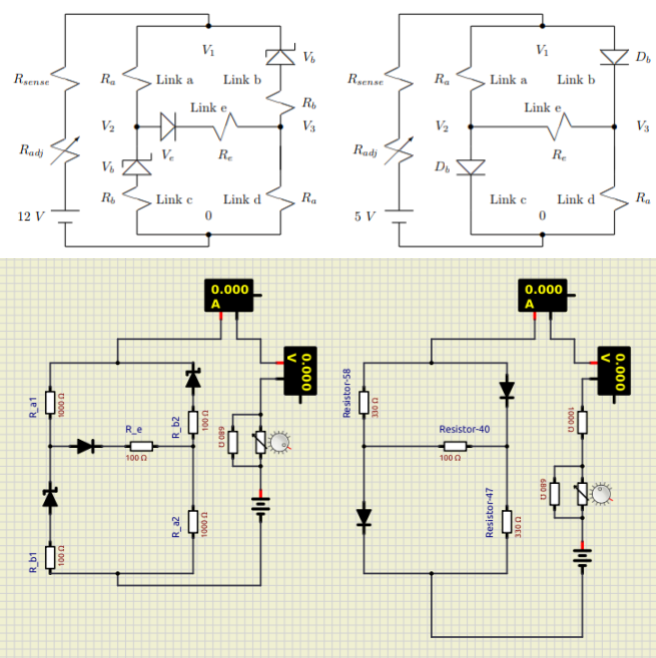
\includegraphics[width=1\linewidth]{sim}
	\caption{2 circuits from \textit{Physical proof of the occurrence of the braess paradox in electrical circuits} \cite{Nagurney2016Braess} implemented in SimulIDE. The left utilizing 2 Zener Diodes, and the other that's similar, but utilizing Diodes only.}
	\label{fig:simulation}
\end{figure}

\bibliographystyle{apalike}
\bibliography{ref.bib}

\end{document}

%aim for 10 pages add deets